\providecommand{\topdir}{..}
\documentclass[../main.tex]{subfiles}

\ifSubfilesClassLoaded{
  \externaldocument[main-]{../main}
  \setcounterref{chapter}{main-chap:conclusion}
  \addtocounter{chapter}{-1}
}{}

\externaldocument{\subfix{../00_front_matter/front_matter}}
\externaldocument{\subfix{../01_introduction/introduction}}
\externaldocument{\subfix{../02_lorenz96/lorenz96}}
\externaldocument{\subfix{../03_rayleigh_benard/rayleigh_benard}}
\externaldocument{\subfix{../04_tendencies/tendencies}}
\externaldocument{\subfix{../05_evaluation/evaluation}}
\externaldocument{\subfix{../07_appendix/appendix}}

\begin{document}

\ifSubfilesClassLoaded{
    \frontmatter
    \tableofcontents
    \mainmatter
}{}

\chapter{Discussion} \label{chap:conclusion}
\setlength{\epigraphwidth}{.45\textwidth}
\epigraphhead[0.1\textheight]{
    \epigraph{
        God does not care about our mathematical difficulties; He integrates
        empirically.
    }{
        Albert Einstein, quoted by Leopold Infeld in
        \emph{Quest: an autobiography}, 1941
    }
}

In \crefrange{chap:rayleigh_benard}{chap:evaluation}, I presented a complete
proof of concept for data-driven parametrisation in \rb{} convection, from the
initial formulation of the problem to the assessment of the parametrised model
in an online setting. In the final chapter of this thesis, I will discuss in
greater detail the issues of coarse model instability (\cref{sec:instability})
and subgrid tendency predictability (\cref{sec:improve_prediction}), suggesting
possible remedies to be experimented with in future work. In
\cref{sec:tendency_explanation}, I will argue that the unusual height-dependent
subgrid tendency correlations observed in \cref{chap:tendencies} are physically
reasonable, justifying their use as the bases for data-driven parametrisation
schemes. To end the discussion, I will identify the outstanding questions that
could be addressed in the future by using and extending the computational tools
developed in this work (\cref{sec:conclusion_unanswered_questions}) and draw
a set of final conclusions from this work (\cref{sec:conclusion}).


\section{Preventing coarse model instability}
\label{sec:instability}
One of the earliest issues encountered in this work was the potential for
low-resolution models to become numerically unstable, making it difficult to
obtain a baseline for evaluating parametrised models. Aside from the need for
a baseline, it seems unlikely that a simple parametrisation scheme like the one
developed in \cref{chap:tendencies} would have improved the skill of a
coarse model on the brink of instability. Since this work was not concerned
with accurately representing physical reality, I chose to artificially add
hyperviscosity terms to the equations. Another option for future work could be
to use stress-free boundary conditions on the top and bottom plates (i.e.,
$w(z=0,1) = \partial u/\partial z|_{z=0,1} = 0$) rather than the no-slip
condition. This could reduce the large near-wall temperature and velocity
gradients that often triggered instability at low resolutions.

However, when modelling real-world systems such as the atmosphere, one does
not have the freedom to simply alter the governing equations. Successful
data-driven parametrisation in these cases will depend on the careful choice of
the numerical methods used to discretise and solve the equations such that
the underlying coarse model is stable, even if it is inaccurate. Futher work
with the \rb{} system should investigate whether other types of solvers
(finite difference/volume/element, etc.) are more suitable.


\section{Strategies for improving subgrid tendency prediction}
\label{sec:improve_prediction}
% § Alternative approaches in literature (Alieva, Gentine papers)
Another obstacle to data-driven parametrisation for spatially continuous
problems is that there is a very large number of possible subgrid tendency
predictors. For \rb{}, one not only has the three prognostic variables, but
also their derivatives to arbitrary order in the two spatial directions. The
position-dependence of the subgrid tendency statistics was a further
complication, adding $z$ to the list of predictors. One could even use
spatially or temporally nonlocal predictors (i.e., the values of the variables
at nearby points in space or previous time steps)---a possibility that was not
even considered in this work. It would be impossible for a human to explore
every possible combination. Supervised machine learning algorithms, discussed
briefly in \cref{sec:data_driven}, are much better-suited to regression
problems with large numbers of predictors and could potentially capture hidden
and/or nonlinear relationships between these predictors and the subgrid
tendencies. There is no doubt, however, that this work was limited by the
simplicity of the predictors and regression models that were considered, and
future work using more sophisticated statistical models may indeed have greater
success without needing to resort to machine learning.

This work was further limited by its use of purely deterministic
parametrisation schemes despite the existence of considerable residuals
in the subgrid tendency regressions
\crefrange{fig:theta_subgrid_vs_pred_tend}{%
fig:w_subgrid_vs_pred_tend}. Stochastic parametrisation, discussed in
\cref{sec:stochastic}, has the potential to reduce mean-state model
biases by emulating the observed residuals. With the tools I have developed for
the \rb{} problem, it would be relatively straightforward to experiment with
various stochastic perturbations of the existing deterministic scheme
\cref{eqn:scheme}, beginning with those that have been tested for
Lorenz '96 (see \cref{sec:l96_statmodels}). This would include the use
of time-correlated (e.g., AR(1)) noise to reflect the persistence (memory)
of the subgrid tendencies.


\section{Physical explanation of subgrid tendency correlations}
\label{sec:tendency_explanation}
Despite the difficulties described in \cref{sec:improve_prediction}, the joint
histograms in \cref{chap:tendencies} gave clear evidence of subgrid tendency
predictability in the near-wall regions. In this section, I argue that
(at least) the correlations involving the $\theta$ subgrid tendency can
be physically explained and are not spurious. As a reminder, the results in
question are:
\begin{enumerate}
    \item The negative correlation between the $\theta$ subgrid tendency and
        $w$ near $z=0,1$,
    \item The positive correlation between the $\theta$ subgrid tendency and
        $\partial u/\partial x$ near $z=0$ and the negative correlation near
        $z=1$, and
    \item The negative correlation between the $\theta$ subgrid tendency and
        the $\theta$ tendency predicted by the coarse model, near $z=0,1$.
\end{enumerate}

I attribute these to the coarse-graining step, which, in the process of
smoothing the temperature field, widens the thermal boundary layer considerably
(compare \cref{fig:coarse_graining_example}a to
\cref{fig:coarse_graining_example}c). On the one hand, there is little change
in boundary layer thickness between the coarse state at time $t$ and the true
coarse state at time $t + \delta t$ because the latter is obtained by first
applying the fine model to the fine state at time $t$ (\cref{itm:fine_model})
and then coarse-graining (\cref{itm:coarse_grain}). This means that the true
coarse tendencies (\cref{itm:true_tend}) are close to zero in the boundary
layers. On the other hand, the coarse model prediction for time $t + \Delta t$
is obtained by first coarse-graining the fine state at time $t$
(\cref{itm:coarse_grain}) and \emph{then} applying the coarse model
(\cref{itm:coarse_model}). At the high Rayleigh number used here ($\rayleigh =
10^9$), advection in the coarse model immediately begins to thin out the
unusually thick boundary layers.

\cref{fig:tendency_explanation} gives a cartoon illustration of the effect of
advection on the temperature field. Consider the bottom left green dot,
which is located near the lower wall, at the base of a rising convection
plume. At this point, the vertical velocity $w$ is positive, and fluid is
rushing inwards from the left and right, making $\partial u/\partial x$
negative. The aforementioned widening of the thermal boundary layer by
the coarse-graining operation has effectively created a large mass of warmer
fluid beneath; this is advected upwards in the coarse model, meaning that
the coarse model predicts a positive tendency $\partial\theta/\partial t$
at the green dot. As explained in the previous paragraph, the true value of
$\partial\theta/\partial t$ is closer  to zero at this point. The subgrid
tendency---the true tendency minus predicted tendency---is therefore negative.

Applying the same logic to the other three green dots in
\cref{fig:tendency_explanation}, as shown by the text boxes, one finds that the
signs of $w$ and the predicted tendency are always opposite to the sign of the
subgrid tendency. The conclusion is that these variables must be negatively
correlated with the subgrid tendency near $z=0,1$. On the other hand, the
$\partial u/\partial x$ has the same sign as the subgrid tendency near $z=0$
(i.e., positive correlation) and the opposite sign near $z=1$ (i.e., negative
correlation). These predictions are all consistent with the observations in
\cref{chap:tendencies}.

It is farily easy to attribute the subgrid $\theta$ tendency correlations to
advection in the coarse model because $\theta$ behaves a tracer that is nearly
conserved by the flow. The velocity field, however, also has a boundary layer
that is widened by the coarse-graining operation, leading me to conjecture that
the subgrid $u$ and $w$ tendency correlations can be explained using a similar
argument. The fact that all the correlations exhibit similar height dependence
lends credence to the conjecture. If this is true, then the fact that $\theta$
is more closely conserved by the flow than $u$ or $w$ could explain why the
correlations for $\theta$ were observed to be consistenly stronger than the
other variables (see, e.g., \cref{tab:r_squared}).

\begin{figure}[ht]
    \centering
    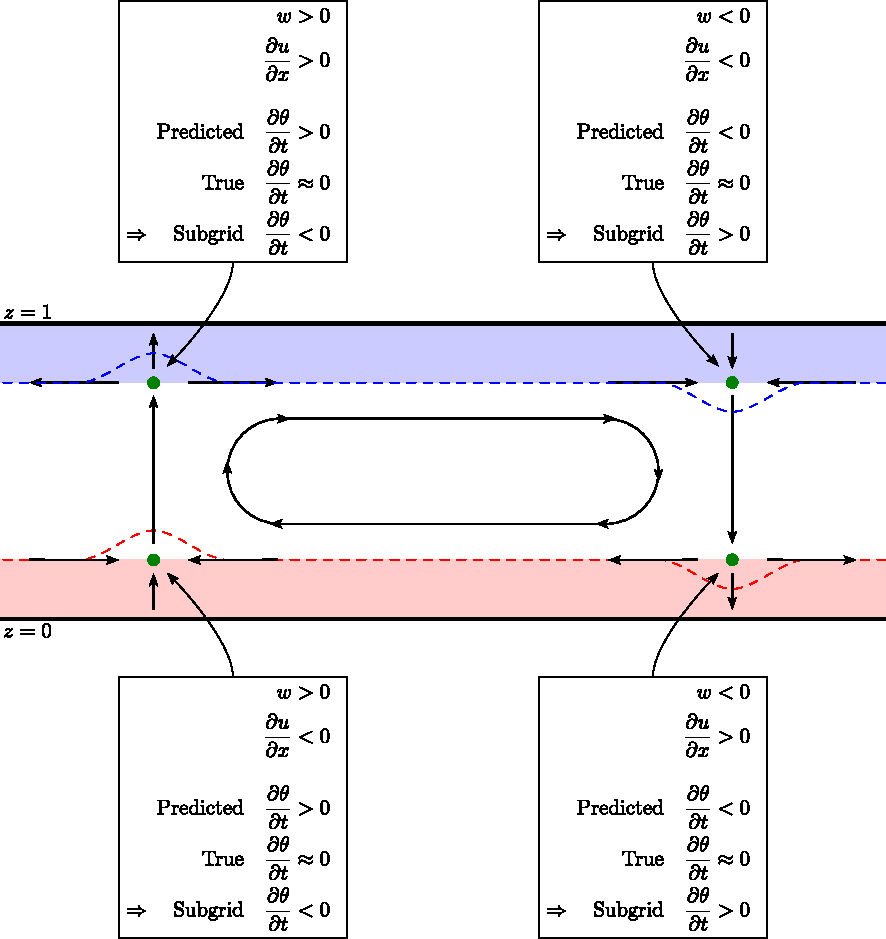
\includegraphics[width=0.8\linewidth]{figures/tendency_explanation.pdf}
    \caption{
        Cartoon illustration of the effect of advection on the coarse-grained
        temperature field when it is evolved using the coarse model. Thick
        horizontal black lines represent the top and bottom domain walls. Black
        arrows represent the velocity field. The warm and cold thermal boundary
        layers are indicated by red and blue shading respectively. Advection
        deforms the isotherms in the boundary layer, which are initially
        approximately flat, in the manner indicated by the dashed red and blue
        lines. The text boxes list the signs of the predictors and predictands
        at the four green dots, demonstrating the claimed correlations.
    }
    \label{fig:tendency_explanation}
\end{figure}

While it is not surprising that the subgrid tendency statistics are
height-dependent, it is interesting that this work was unable to produce
evidence of predictability in the interior of the domain, away from $z=0,1$.
Future work should investigate whether more advanced statistical models and/or
machine learning are able to reveal correlations in this region.


\section{Unanswered questions}
\label{sec:conclusion_unanswered_questions}
The amount of effort this work has devoted to overcoming prerequisite issues
has inevitably limited the scope of its experimentation with actual
parametrisation development and assessment. The positive outcome, however, is
that it has implemented the computational tools needed to undertake further
research with the \rb{} system and made them publicly available for others to
use; see \cref{chap:computations}. There are several worthwhile research
questions that could be addressed using these tools.

The foremost goal for future work is to determine the extent to which the
inclusion of stochasticity and/or memory in parametrisation schemes can improve
their online performance, as well as the optimal method of inclusion. As
discussed in \cref{chap:introduction}, these are topics of considerable
research interest in the context of weather and climate modelling. It would be
possible to include random forcings in a parametrisation either additively or
multiplicatively, and one could also compare the effects of spatially and/or
temporally correlated noise to white noise. Online performance could be
assessed using the same methods as this work: forecast accuracy using the RMSE
of the prognostic variables and time series of domain-averaged metrics, and
long-term statistical accuracy using time averages of the same metrics. It
would be insightful to also test offline performance more thoroughly, perhaps
using the Hellinger distance to measure the agreement between the distributions
of predicted and true tendencies (see \cref{sec:l96_offline_testing}).

A second important goal is to determine each scheme's ability to generalise to
conditions unseen in its training dataset, such as initial conditions with
different numbers of convection cells or changes in Rayleigh number or domain
aspect ratio. The findings could inform the development of parametrisations
for climate models whose effectiveness is robust in warming conditions---an
important goal of modern research.

With a wider variety of statistical models for the subgrid tendencies in
combination with a range of stochastic perturbation schemes (with different
noise amplitudes, correlation times, etc.), it would be possible to determine
whether schemes that perform well offline generally also perform well online,
and whether or not their short-term forecast accuracy is correlated with their
long-term statistical accuracy. These have been topics of for the Lorenz '96
system (see \cref{sec:l96_open_questions}), and an extension to \rb{} could
provide further evidence to aid the selection of parametrisation schemes for
weather and climate models.


\section{Conclusion}
\label{sec:conclusion}
Motivated by previous studies on the Lorenz '96 system and open questions in
weather and climate modelling that call for experimentation in more realistic
test frameworks, I have implemented a complete proof of concept for data-driven
parametrisation in \rb{} convection. Given a high-resolution ``truth'' model of
the flow and a low-resolution baseline model, straightforward mathematical
arguments in \cref{chap:introduction} justified a method for calculating the
subgrid tendency of each prognostic variable---that is, the contribution of
small-scale processes unresolvable by the coarse model to the rate of change of
the large-scale state that it could resolve. The method was implemented in
\cref{chap:tendencies} and involved systematic coarse-graining of a
high-resolution training simulation and time-stepping with the low-resolution
model.

Exploratory analysis in \cref{sec:subgrid_analysis} revealed several
correlations between the subgrid tendencies and the large-scale state of the
coarse model. The correlations were all strongly conditional on vertical
position, appearing to exist only near the top and bottom boundaries of the
domain. The most notable of these was a negative linear correlation between the
subgrid tendency of each variable and the corresponding tendency predicted by
the low-resolution model. A simple parametrisation scheme for predicting the
subgrid tendencies based on this relationship was fitted to the training
dataset and coupled into the low-resolution model to emulate the effect of the
unresolved processes.

Running online, the parametrisation scheme was found to improve the forecast
accuracy of the coarse model, but only for short lead times. It was also found
to improve long-term statistical accuracy, reducing the relative error of some
metrics by as much as one half. The parametrisation was found to introduce
little to no additional overhead computational cost relative to the control.
This work therefore provides, from first principles, evidence that data-driven
parametrisation is a viable method for improving the skill of low-resolution
weather and climate models.

The process of parametrisation development for the \rb{} problem highlighted
subtle technical obstacles that do not apply to simpler systems such as Lorenz
'96. Firstly, coarse models were prone to numerical instability, necessitating
a hyperdiffusive modification of the governing equations. Secondly, the
predictability of the subgrid tendencies was found to depend strongly on the
method used to coarse-grain the high-resolution solutions, and the development
of an an appropriate method was non-trivial. The understanding of these issues
and the development of computational tools to address them is a second major
outcome of this work.

Future work will be able to use and extend the tools established here to
perform further parametrisation experiments, addressing important
unanswered questions that relate to parametrisation in real weather and climate
models. Although it remains an idealised system, \rb{} convection has proven to
be a highly instructive test problem and there are no doubt many more lessons
to be learnt from it in the future.


\ifSubfilesClassLoaded{%
    \emergencystretch=5em
    \printbibliography{}
}{}

\end{document}
